\newpage
\section{Efficiently solvable abstractions}\label{solveable-abstractions}

\begin{displayquote}
  \textsl{Abstractions for efficient control.}
\end{displayquote}

% The control problem can be expensive, especially when there are long horizons, or high discount rates.
% For example, bound, bound. Can

In optimisation for supervised learning we know that
linear models can be solved analytically and convex problems converge quickly.
What makes an RL problem easy to solve? Is there linearity or convexity
within RL problems that we can use to find solutions more efficiently?

% bellman eqn is hard to solve (how hard?)
% Existing solvers of MDPs such as are not efficient: value iteration requires at
% least \href{https://en.wikipedia.org/wiki/EXPTIME}{EXPTIME} iterations,
% policy iteration requires ???, or policy gradients,
% require a ??? amount of computation.
% Yet, recent work \cite{} has shown that MDPs require at least $\Omega(|S|^2|A|).$

While some interesting work has been done exploring convex RL \cite{ODonoghue2012a, Barratt2019},
we choose to explore linear RL.

\subsection{Linear Markov decision problems (LMDPs)}

\begin{displayquote}
\textsl{Why linear MDPs?}
\end{displayquote}

% How are we exploiting linearity?
% Linearisation around the optima? Intuition. How to see this? Stephen!?
% Intuition.

% \subsubsection{Existing linear methods}
%
% The optimal policy of a MDPs can be found be using linear programming.
% Traversing through the (value ??) space, ...?

% many mathematical tools for analysis.
% we know linear systems can be solved efficiently.

% Linear systems are easy to solve. (ref). They have $\mathcal O(n^3)$ complexity.

Imagine if your life were linear, in the sense of effort and achieving goals.
More work equals proportionally more rewards. This makes decision making
a lot more simple. Pick the most rewarding activity, and work hard.

\subsubsection{What do we mean by a linear MDP?}

Do we mean that the value function is a linear function of (say) a policy?
Of the reward function? Of the transition function? Previous researhc has tried to incorporate
linearity into MDPs in a few different ways.

\begin{itemize}
  \tightlist
  \item Todorov constructs a linearised MDP that is linear in the 'control' (a proxy for the policy) \cite{Todorov2006}.
  \item Jin et al. construct a MDP where the value is a linear function of a state-action representation and of a policy embedding \cite{Wang}.
  \item Levine et al. construct a learner that assumes a linear transition function, allowing the use of \href{https://en.wikipedia.org/wiki/Linear%E2%80%93quadratic_regulator}{LQR} solvers \cite{Levine2019}.
  \item Pires et al. construct a factored linear MDP that allows the TD operator to be applied in a lower dimensional space \cite{Pires2016}.
\end{itemize}

Todorov's formulation appears to be the most powerful. By having a linear
relationship between the value and the control, we can easily search for controls that
are optimal. For the rest of this work we will refer to these as LMDPs.

% Saxe el al. observe the power of linearity: \textit{"Consider two standard MDPs
% $M_1 = \{S, A, P, R_1\}$ and $M_2 = \{S, A, P, R_2\}$ which have
% identical state spaces, action sets, and transition dynamics but differ in their
% instantaneous rewards $R_1$ and $R_2$. These may be solved independently to
% yield value functions $V_1$ and $V_2$. [If the problems were linear then] the value function of the MDP
% $M_{1+2} = \{S, A, P, R_1 +R_2\}$, whose instantaneous rewards are the sum of the
% first two, [would be] $V_{1+2} = V_1 + V_2$.} \cite{Saxea}

\subsubsection{Constructing a LMDP}

\begin{figure}[h!]
  \centering
  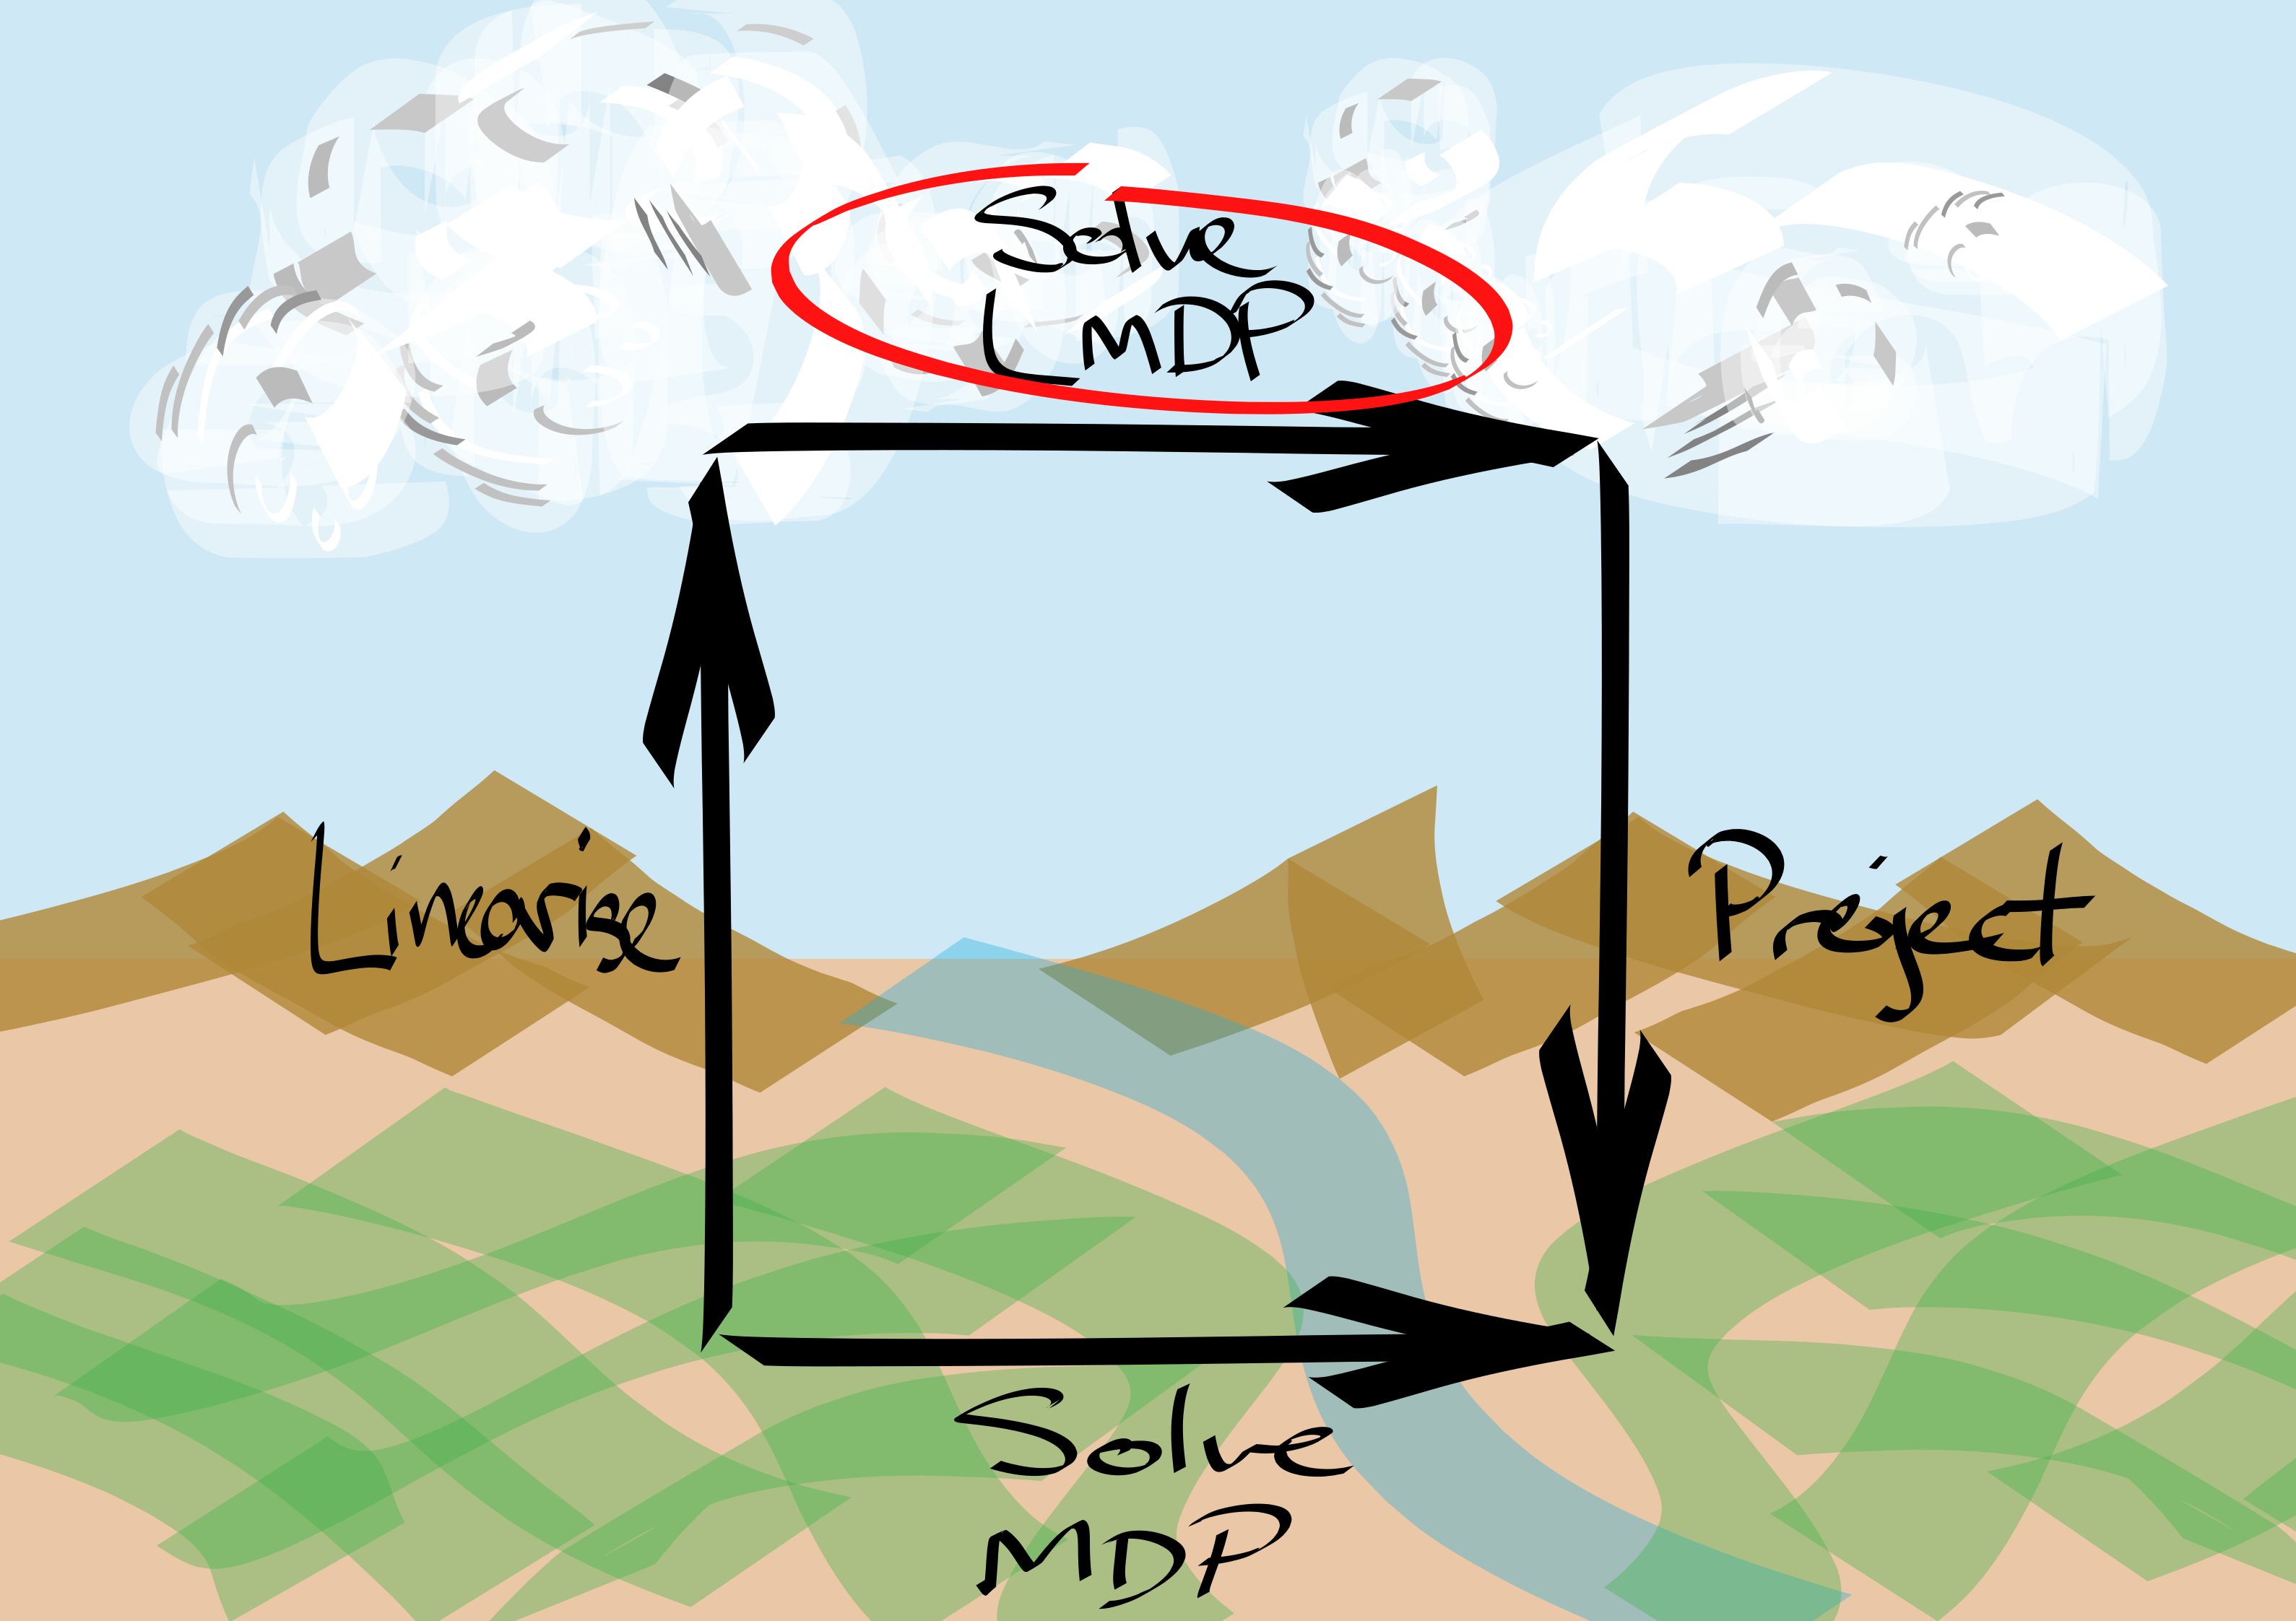
\includegraphics[width=0.6\textwidth,height=0.3\textheight]{../../pictures/drawings/abstract-representations-solve.png}
  \caption{Solving the LMDP}
\end{figure}

To build a LMDP that acts similarly to a MDP, Todorov \cite{Todorov2006} incorporate a few changes to the typical MDP setting;

\begin{itemize}
\tightlist
  \item
  allow the agent to pick actions in the space of possible transitions, which they name 'controls', $u: S \to S$.
  \item
  ensure that chosen controls are possible under the given transition function, a new reward is added.
  Controls are rewarded if they are close to the 'unconstrained dynamics', $p(s' | s)$.
  \item
  maximise the exponentiated cumulative rewards.
  $\mathop{\text{max}}_{u} \mathop{\mathbb E}_{\zeta \sim D(u)} e^{R(\zeta)}$ \cite{EricWarrenFox2016} (rather than maximizing the cumulative reward).
\end{itemize}

The intuition behind these changes seems to be; we have allowed the learner to pick an arbitrary control.
This simplifies the optimisation problem. But, now the learner might pick a control that is not possible
under the given transition function. So we incentivise controls that are close to the underlying dynamics.

\begin{displayquote}
\textit{"It is reminiscent of a linear programming relaxation in integer programming"} \cite{Todorov2009}.
\end{displayquote}

% What is the relationship to other action embedding strategies? {\color{red}!!!!!}

% Why did they need these tricks? Which ones were necessary / sufficient? !!!!!!!

% formal definition
Putting these changes together, a linear Markov decision process can be formulated as;
LMDP = $\{S, U, p, q, \gamma\}$. Where $S$ is the state space, $U$ is the space of possible controls (i.e. any transitions),
$p: S \to S$ is the unconditioned dynamics, and $q \in \mathbb R^{|S|}$ is state rewards.
Our goal is to find the control, $u: S \to S$, that gives the highest exponentiated cumulative reward $z \in \mathbb R_+^{|S|}$.

\begin{align}
\log z_{u^{* }}(s) &= \mathop{\text{max}}_{u} q(s) - \text{KL}(u(\cdot| s) \parallel p(\cdot | s)) + \gamma \mathop{\mathbb E}_{s' \sim u(\cdot | s)} \log z_{u}(s') \tag{1}\\
u^{* }(\cdot | s) &= \frac{p(\cdot | s)\cdot z_{u^{* }}(\cdot)^{\gamma}}{\sum_{s'} p(s' | s) z_{u^{* }}(s')^{\gamma}} \tag{2}\\
z_{u^{* }} &= e^{q(s)}\cdot P z_{u^{* }}^{\gamma} \tag{3}
\end{align}

By definition, a linearised Bellman equation can be constructed (1). After some algebra,
it can be shown that the optimal policy has the form in (2).
Most importantly! We can solve for the value of the optimal control by solving the linear equation in (3).
(see \ref{lmdp-derivation} for further explanation and a derivation of a LMDP)

\begin{displayquote}
\textsl{Let's try and understand this LMDP has been constructed.}
\end{displayquote}

\subsubsection{The unconstrained dynamics and state rewards}

\begin{displayquote}
\textsl{What do $p$ and $q$ do?}
\end{displayquote}

Rather than state-action rewards $r: S \times A \to \mathbb R$, we have state rewards $q: S \to \mathbb R$.
How can state rewards direct behaviour? They can't, and they can. State rewards are not capable of drectly giving rewards for actions taken.
Rather, the action dependent part of the reward is captured by the KL divergence between
the control and the unconstrained dynamics (this relationship is shown in \ref{unconstrained-dynamics-reward}).
But, they do implicitly direct behaviour through their presence in the exponentiated value function $z_{u^{* }}$.

While it may seem intuitive to think of the unconstrained dynamics as the expected result of using random policy
$p(s' | s) = \int_a P(s' | s, a)U(a|s)$ (a random walk using the transition function).
This turns out to be wrong. The unconstrained dynamics are responsible for rewarding actions.

\subsubsection{The optimal policy}

\begin{displayquote}
\textsl{What can we interpret about the form of the optimal control?}
\end{displayquote}

\begin{align*}
u^{* }(\cdot | s) &= \frac{p(\cdot | s)\cdot z_{u^{* }}(\cdot)^{\gamma}}{\sum_{s'} p(s' | s) z_{u^{* }}(s')^{\gamma}}
\end{align*}

Interpreting the equation above, the optimal control is the control that transitions to new state, $s'$, with a
probability proportional to the discounted exponentiated value of that state, $z(s)$.
That seems reasonable, and is closely related to the RL as inference framework \cite{Levinea},
which picks actions with probability proportional to their exponentiated $Q$ values.

\begin{align*}
\pi(\cdot|s) \propto e^{Q(s, \cdot)}
\end{align*}

\subsubsection{Solving for the optimal value}\label{solve-lmdp}

\begin{displayquote}
\textsl{What can we interpret about the form of the value estimate?}
\end{displayquote}

\begin{align*}
z_{u^{* }} &= e^{q(s)}\cdot P z_{u^{* }}^{\gamma}
\end{align*}

In the undiscounted case (aka first exit case), where $\gamma=1$, this turns into an eigen value
problem $z = QPz = Az$. In the discounted case, the exponentiated value, $z$, is guaranteed to converge \cite{Todorov2009}.

\subsection{Solving a MDP}\label{construct-lmdp-from-mdp}

\begin{figure}[h!]
\centering
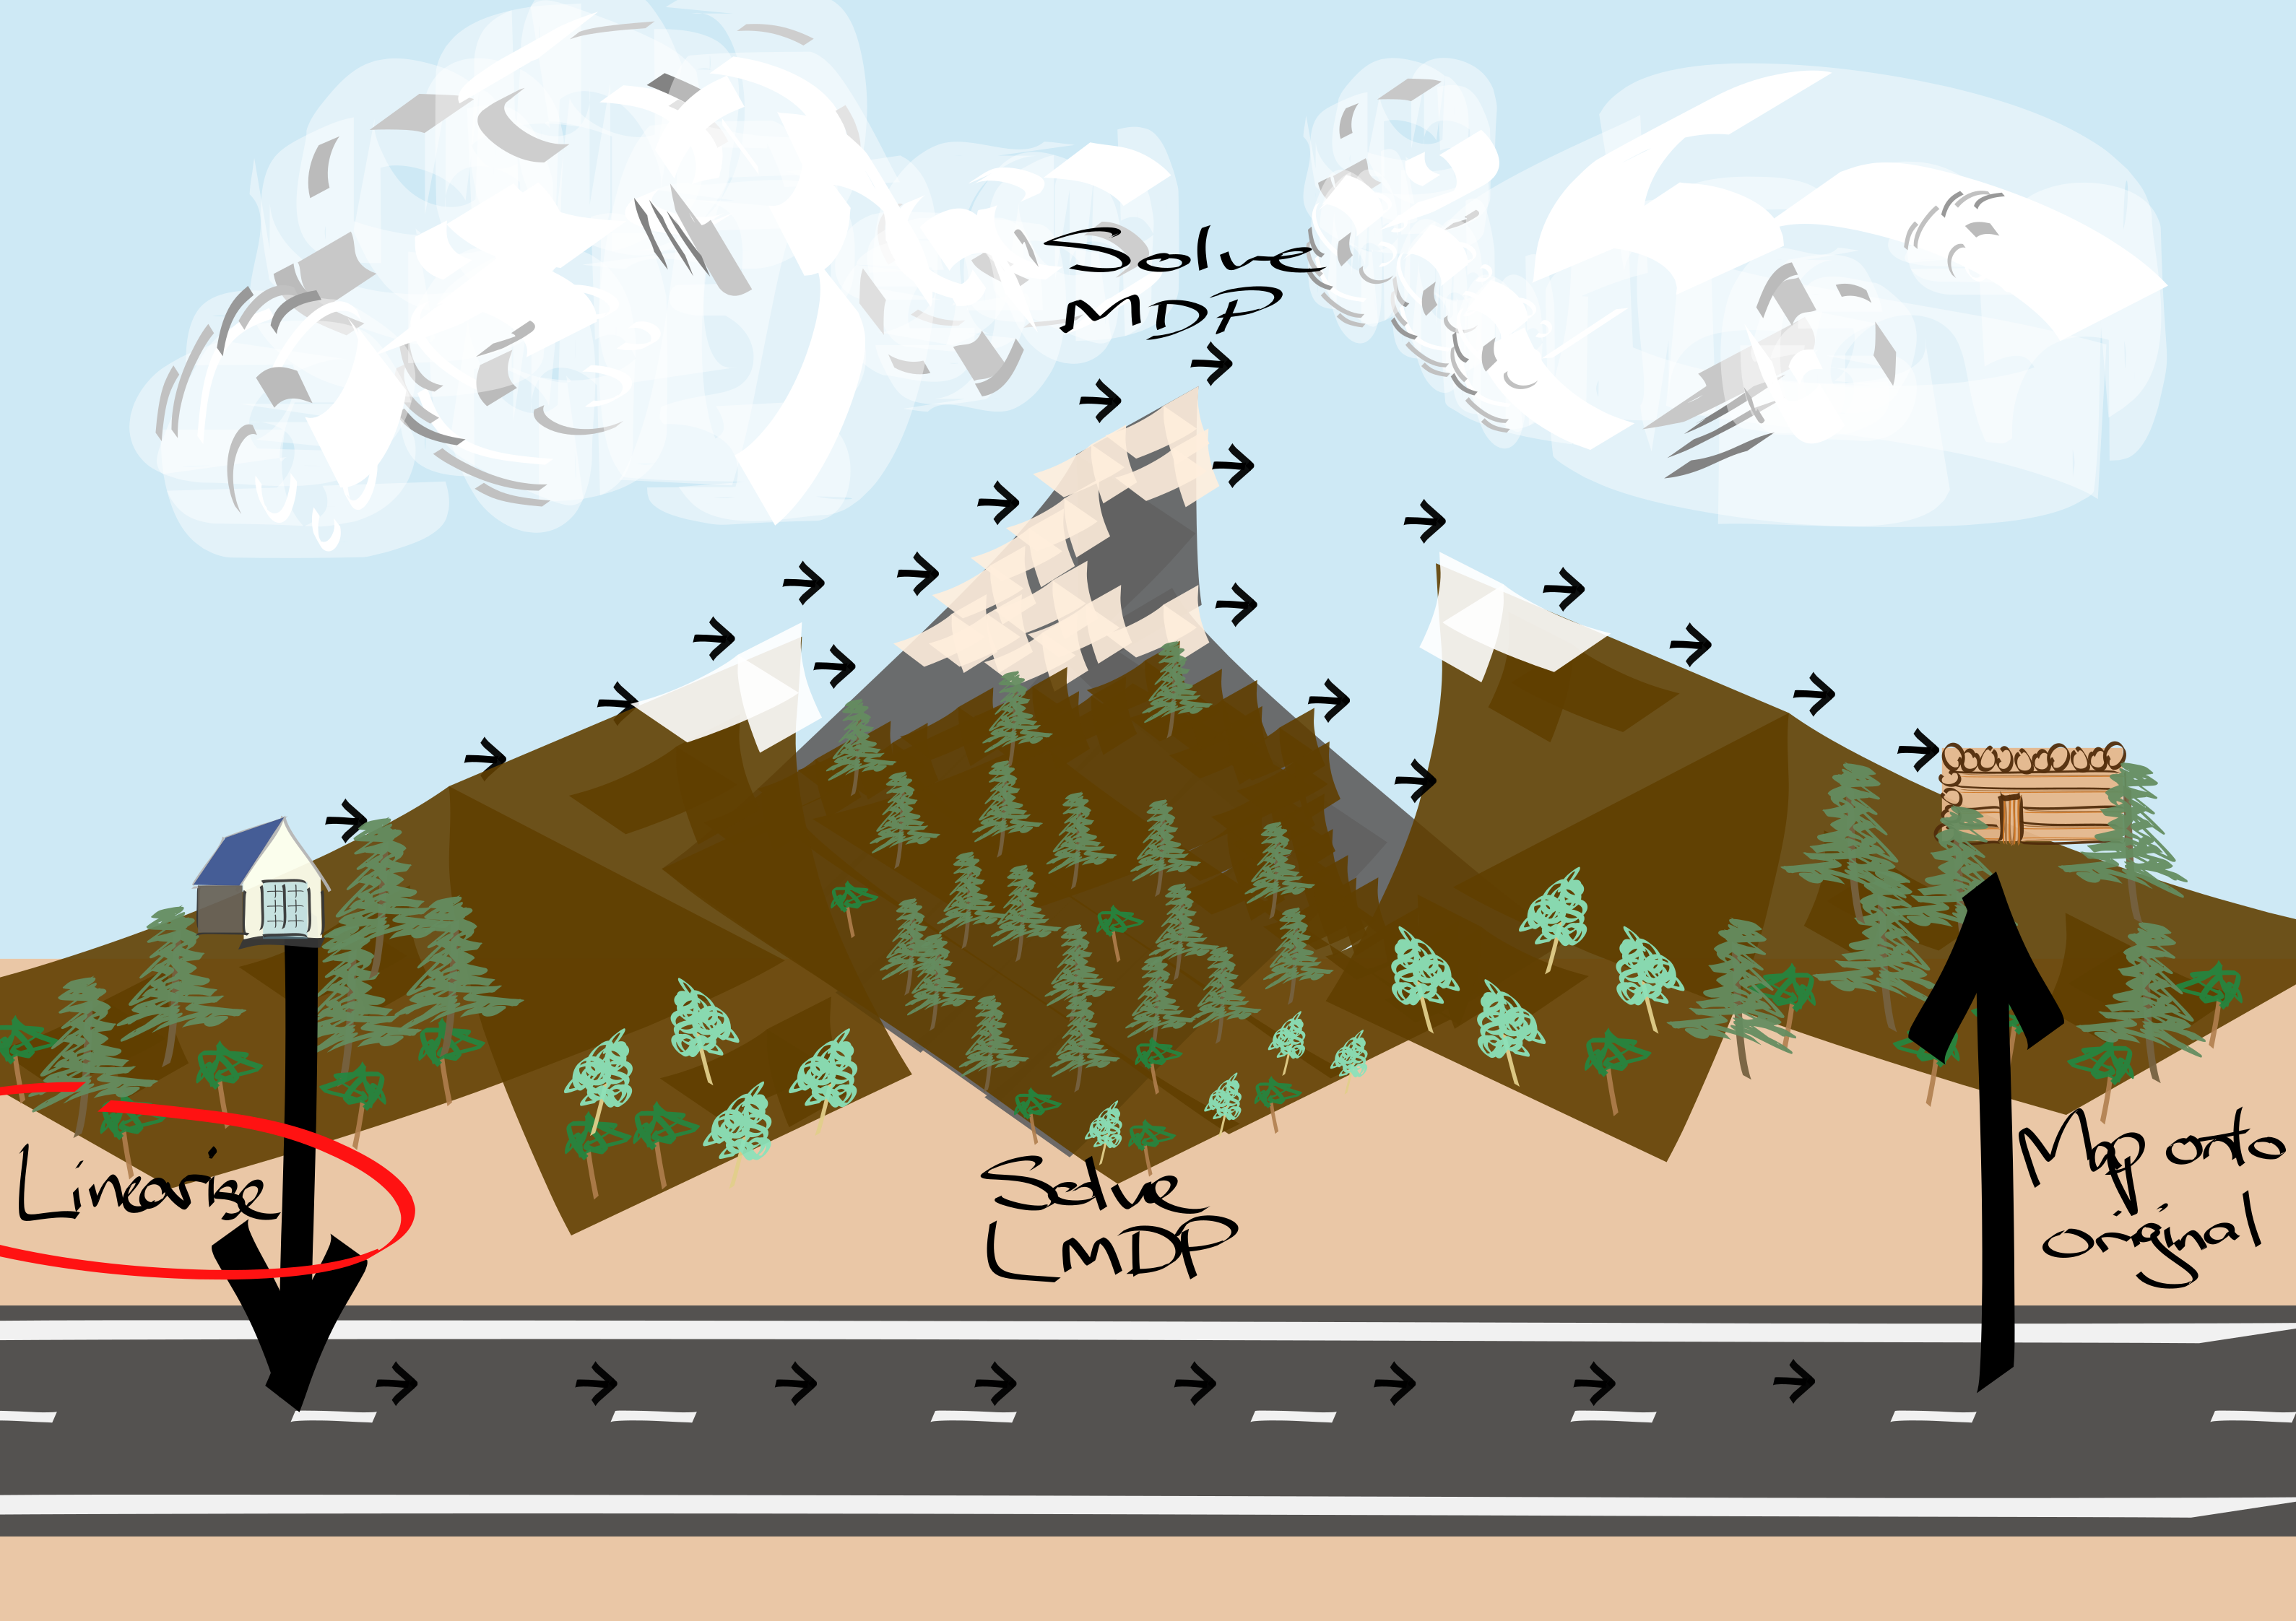
\includegraphics[width=0.6\textwidth,height=0.3\textheight]{../../pictures/drawings/abstract-representations-linear.png}
\caption{Solving a MDP}
\end{figure}

\begin{displayquote}
\textsl{So, LMDPs can be easily solved. But how does solving a LMDP help us solve a MDP?}
\end{displayquote}

We need a way to transform a MDP into a LMDP, while preserving the
`structure' of the original MDP. But what do we mean by a MDP's structure?
According \cite{Todorov2009}, the LMDP should be able to represent the same \ref{state-reward-rep} as the original MDP,
and give the the same \ref{unconstrained-dynamics-reward} was the original MDP.

\begin{align*}
\forall s, s' \in S, \forall a \in A, \exists u_a& \;\;\text{such that;} \\
P(s' | s, a) &= u_a(s'|s)p(s'|s) \tag{transition dynamics} \label{state-reward-rep} \\
r(s, a) &= q(s) - \text{KL}(P(\cdot | s, a) \parallel u_a(\cdot| s) ) \label{unconstrained-dynamics-reward} \tag{rewards}
\end{align*}

% "We do not yet have theoretical error bounds but have found the approximation to be very accurate in practice" \cite{Todorov}

So, given a reward function, $r$, and a transition function, $P$,
(from an MDP), we can use the \ref{state-reward-rep} and \ref{unconstrained-dynamics-reward}
to solve for the unconditioned dynamics $p$ and a state reward $q$.
This transformation, from $P, r \to p, q$ requires $|S| \times |A|$ computations, as for each state in the
MDP we need to satisfy constraints for each action. For a derivation and explanation see appendix \ref{mdp-Linearisation}.

However, an important condition missing!
We should preserve the value of optimal actions (as discussed in \ref{efficient-control}).
Alternatively, we might settle for preserving the optimal policy.

\begin{align*}
\forall s, s' \in S, \forall a \in A, \forall \pi \in \Pi \\
z_{u_{\pi}}(s) = e^{V_{\pi}(s)} \label{value-preserved}\tag{value} \\
P(s'|s, a) \cdot \pi^{* }(a|s) = u^{* }(s'|s) \label{opt-policy-preserved}\tag{optimal policy}
\end{align*}

Where $z_{u_{\pi}}$ is the value (as evaluated by the LMDP) of the control $u_{\pi}(s'|s) = P(s'|s, a) \cdot \pi(a|s)$, and $V_{\pi}$ is the expected return of policy $\pi$ as evaluated by the original MDP.

It seems that Todorov hopes that the constraints \ref{state-reward-rep}, \ref{unconstrained-dynamics-reward},
will be sufficient to give \ref{value-preserved}, \ref{opt-policy-preserved}. But he does not prove it.
This is problem that we will return to in \ref{paths}.

\subsection{Lifting the optimal LMDP policy}\label{lift-mdp}

\begin{figure}[h!]
\centering
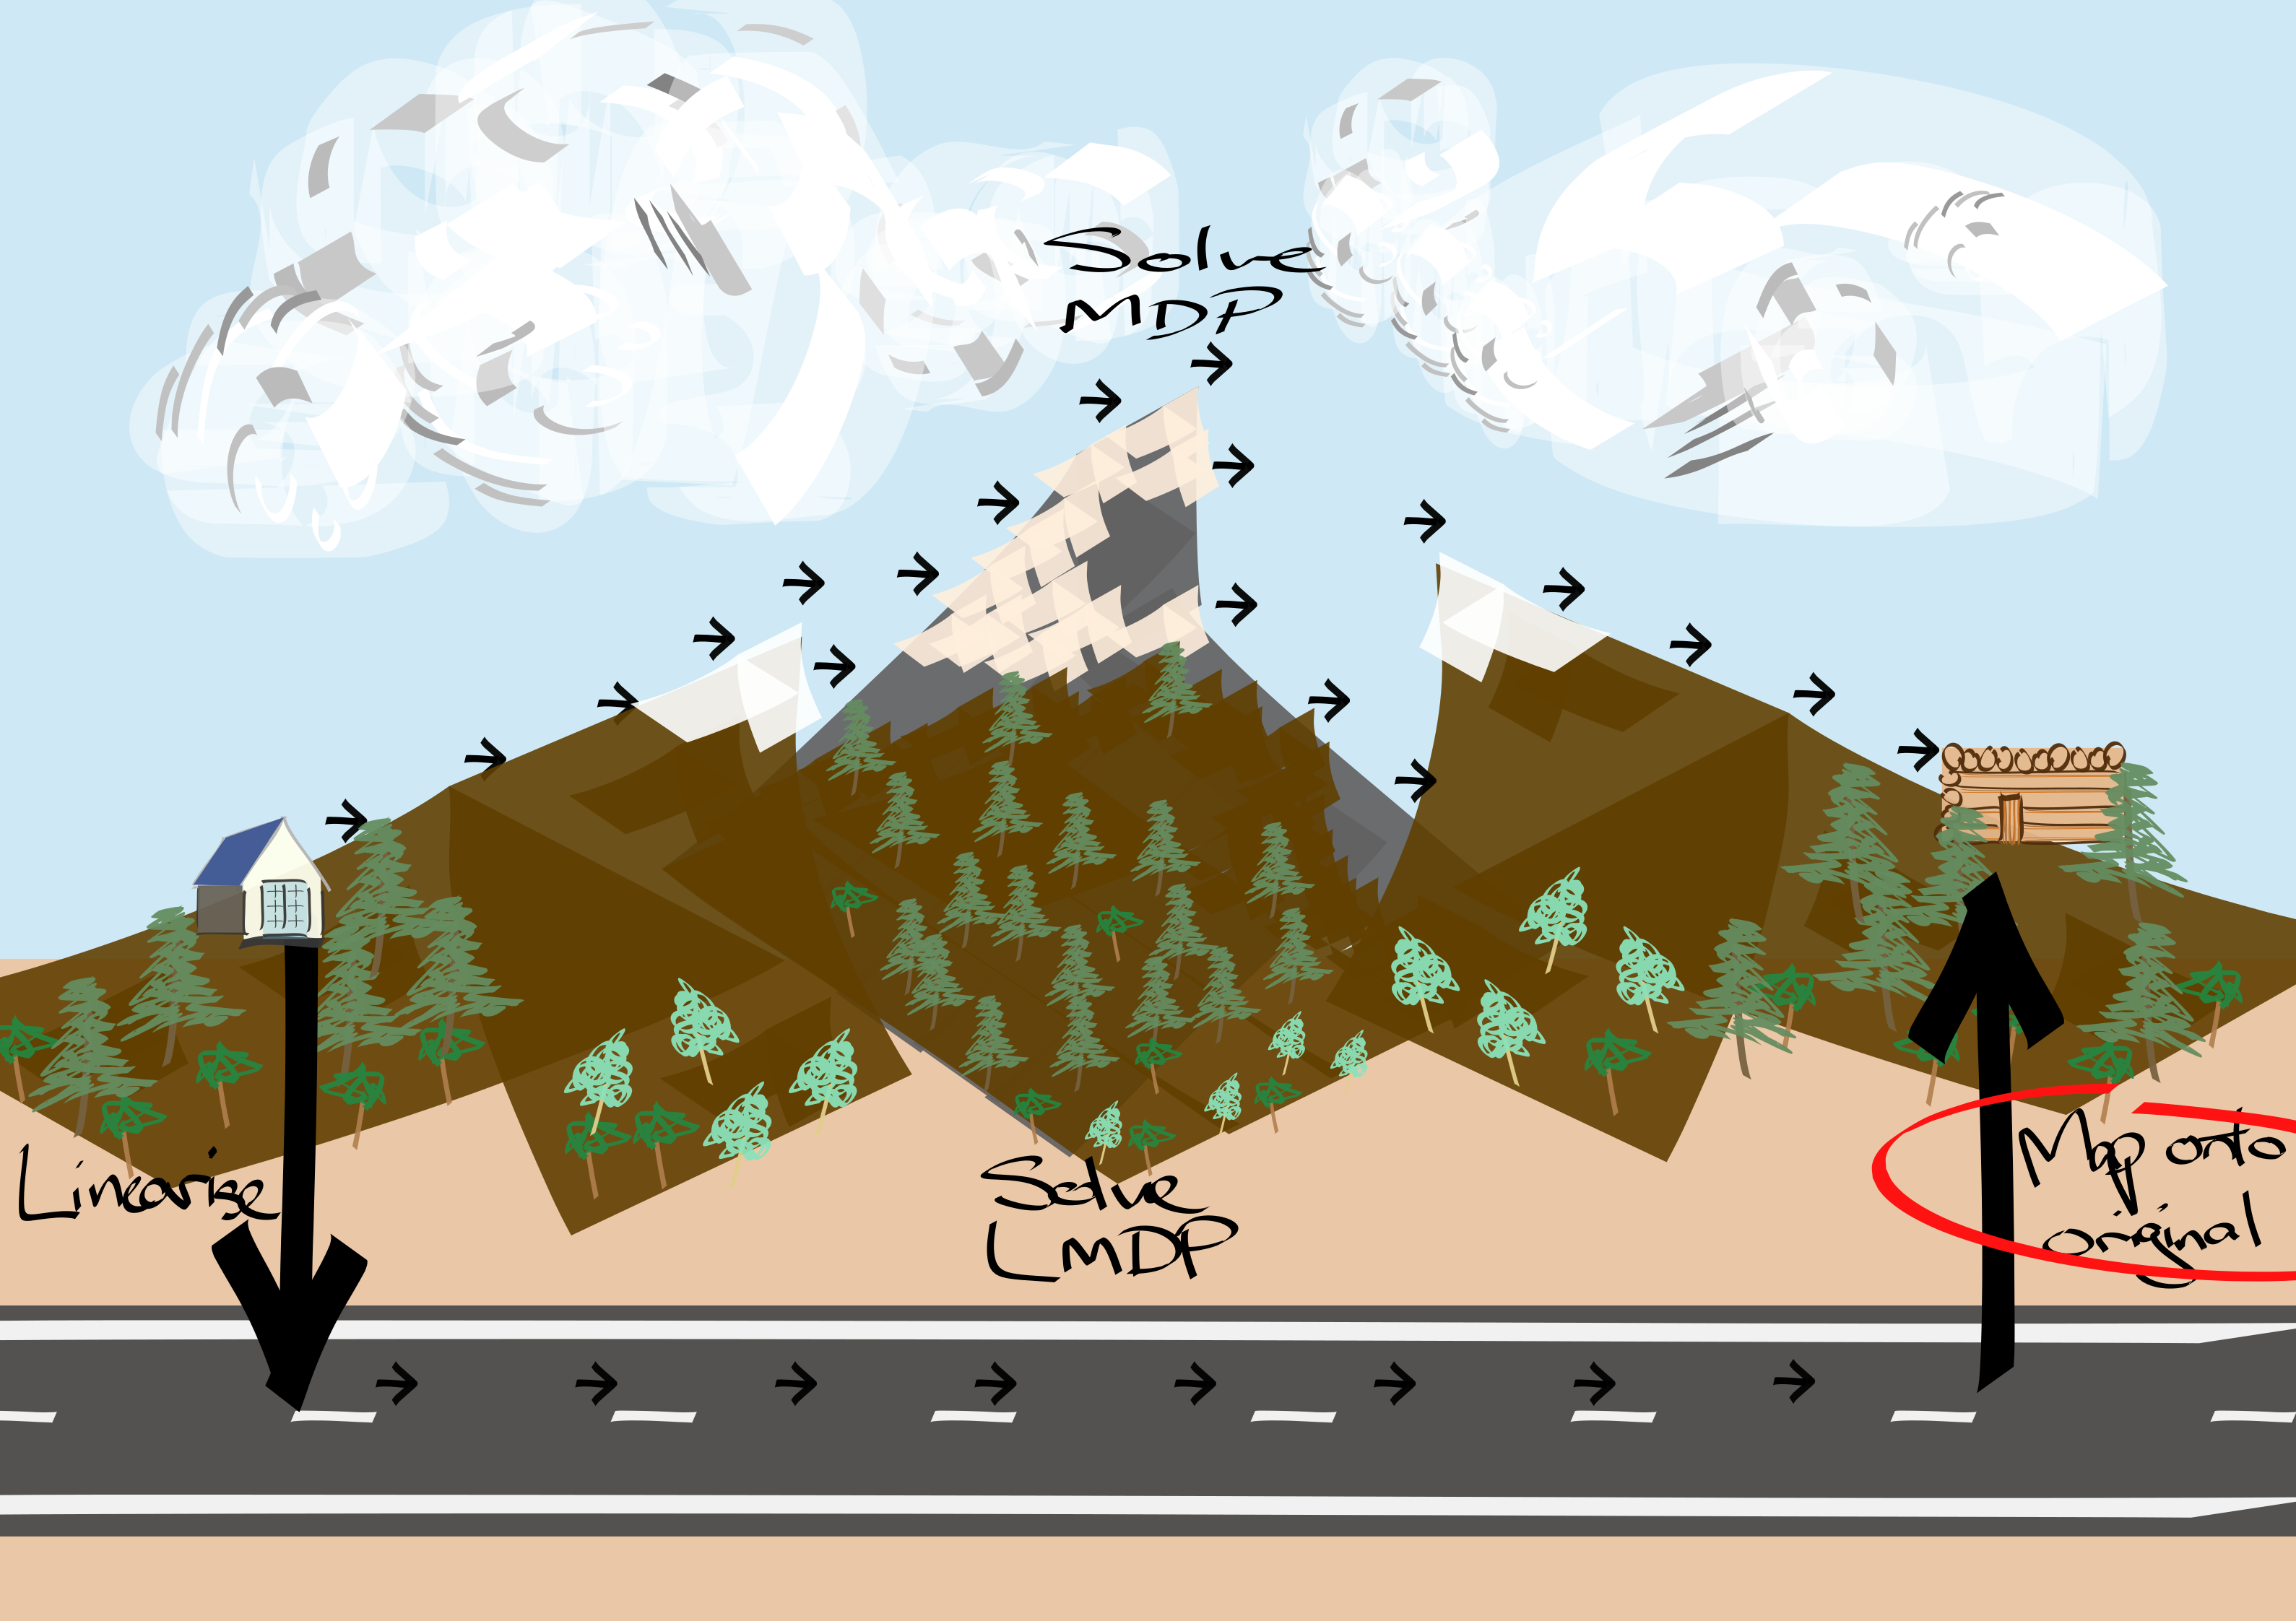
\includegraphics[width=0.6\textwidth,height=0.3\textheight]{../../pictures/drawings/abstract-representations-project.png}
\caption{Lifting the LMDP's solution to the MDP}
\end{figure}

\begin{displayquote}
\textsl{How can we use the optimal control, $u^{* }$, to construct a policy that is optimal in the original MDP, $\pi_{u^* }$?}
\end{displayquote}

The LMDP has disentangled the search for the optimal controls (solve the LMDP) (go to this or
that state) and the search for the optimal policy (how to actually
realise that control).

This decomposition is reminiscent of goal conditioned approaches to hierarchical RL.
Where a higher level agent gives goals (go to this or that state) to a lower level
agent, who must figure out how to achieve that goal \cite{Vezhnevets2017}.

This decomposition within the LMDP can be seen the optimal control decoding
step (currently being considered). We know which
states we want to be in, the $z^{* } / u^{* }$, from solving the LMDP, but,
we do not know how to implement those controls with the actions we have available in the original MDP.
We can formulate this problem as;

\begin{align}
P_{\pi}(\cdot | s) = \sum_a P(\cdot | s, a) \pi(a | s) \\
\pi = \mathop{\text{argmin}}_{\pi} \text{KL}\Big(u(\cdot | s))\parallel P_{\pi}(\cdot | s)\Big)
\end{align}

We would hope that the knowledge of $u^{* }$ would make it easy to find the optimal actions.
But, this optimisation problem has very little structure for us to exploit.
In the worst case it has complexity $\mathcal O(|S|^2|A|)$ (which is the same as solving a MDP).

\begin{center}\rule{0.5\linewidth}{\linethickness}\end{center}

We have now built a way to solve a MDP with a LMDP.
We have a method to transform a MDP to a LMDP \ref{construct-lmdp-from-mdp}.
We can solve the LMDP \ref{solve-lmdp}.
And finally, we can lift the solution to the original MDP \ref{lift-mdp}.
Let's try it out.

\subsubsection{Optimality of solutions via LMDPs}\label{paths}

\begin{quote}
\textsl{Do these two paths lead to the same place?}
\end{quote}

One of the main questions we have not addressed yet is; if we solve the
MDP directly, or we linearise then solve then lift, do we end up in the same
place? This is a question about the sub-optimality of our abstraction \ref{near-optimal-abstraction}. Can
our abstraction approximately represent (and find) the same solutions that the
original can? We can formalise this question as the difference between the optimal values or optimal policies.

\begin{align*}
\epsilon &= \parallel Q_{\pi^{* }} - Q_{\pi_{u^{* }}} \parallel_{\infty}
\end{align*}

We answer this question using experiments, described in figures \ref{fig:ltd} and \ref{fig:opt-control}.

\begin{figure}
\centering
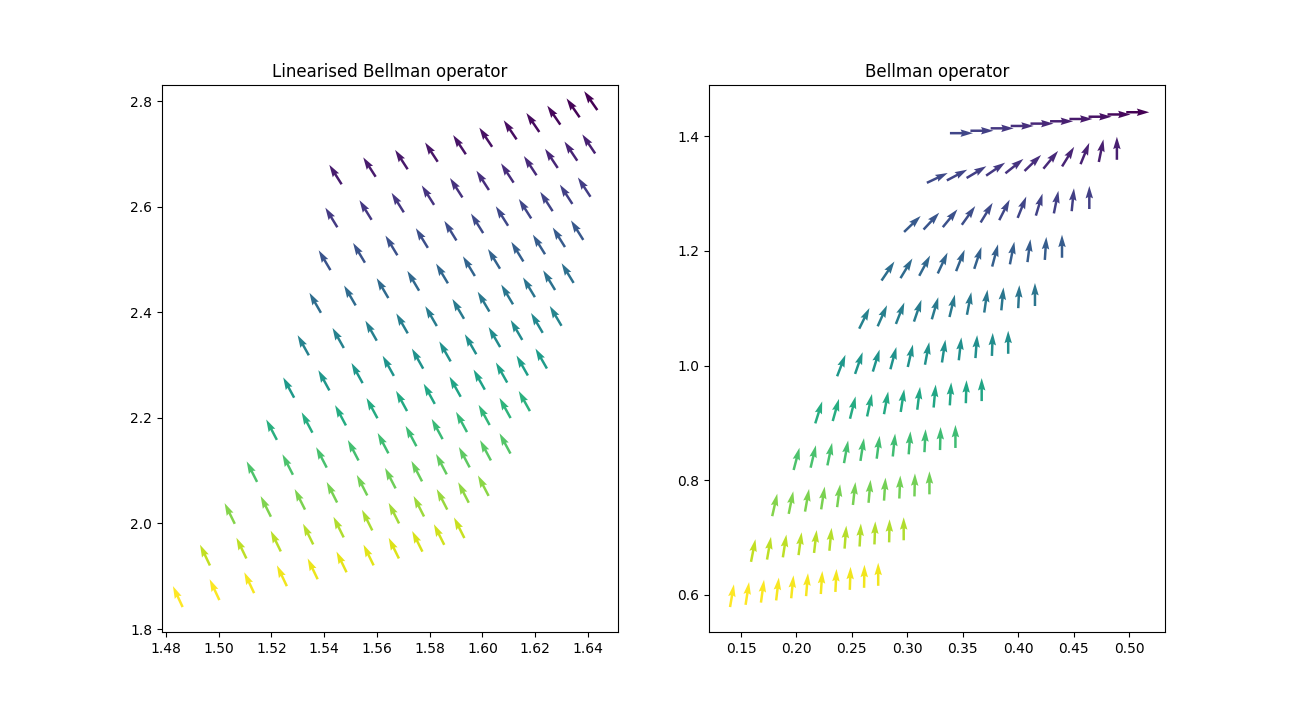
\includegraphics[width=0.75\textwidth,height=0.5\textheight]{../../pictures/figures/LBO_BO.png}
\caption{For the same MDP, shown is a comparison of the linear temporal difference operator (left), versus the true, Bellman, temporal difference operator (right). As expected, the temporal difference operator points towards the optimal value. But, the linear temporal difference operator points elsewhere.}
\label{fig:ltd}
\end{figure}

\begin{figure}
\centering
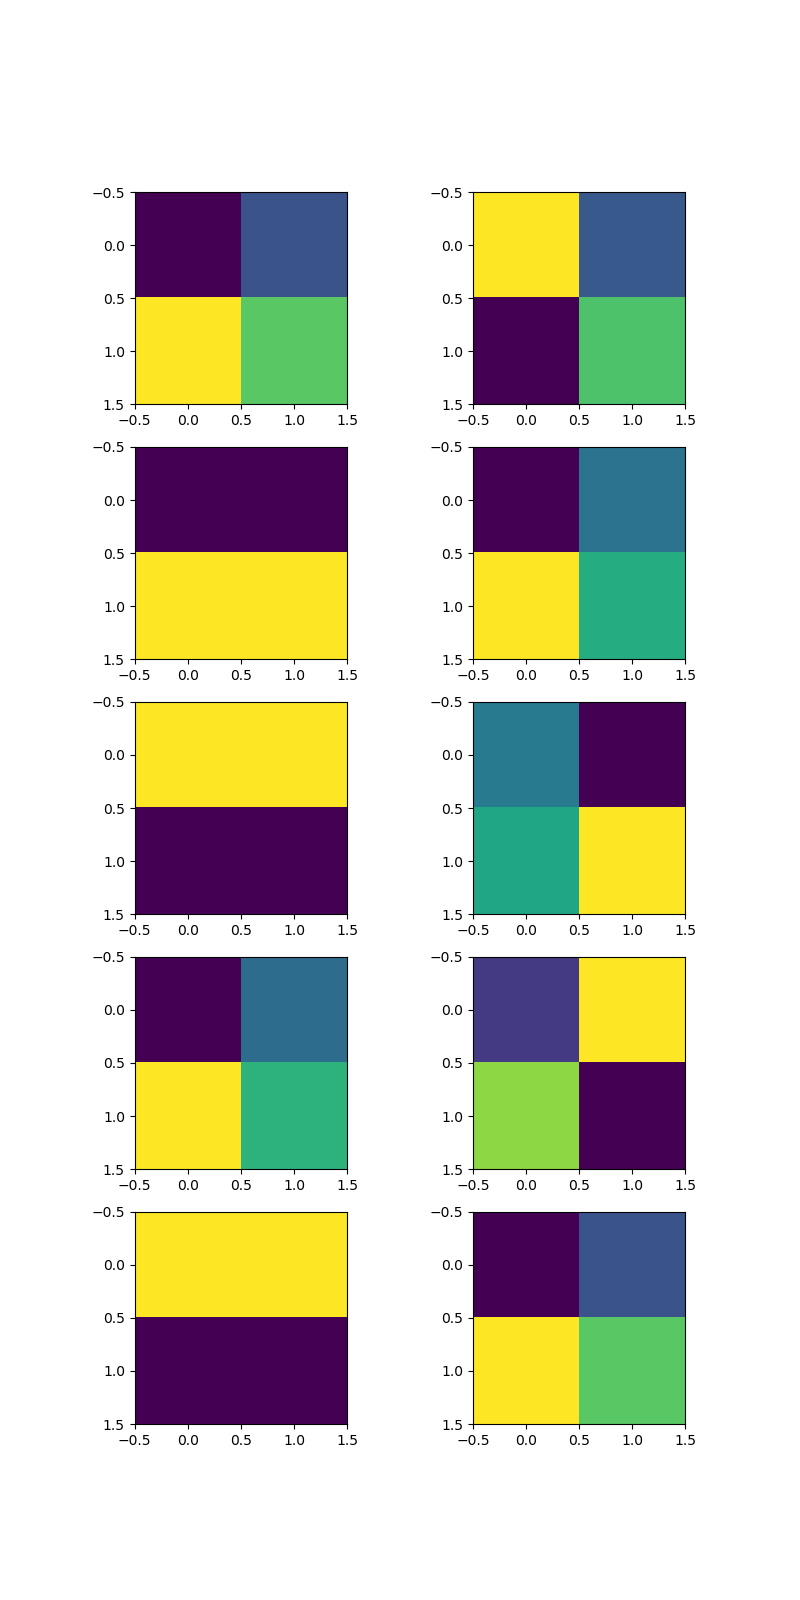
\includegraphics[width=0.5\textwidth,height=0.75\textheight]{../../pictures/figures/lmdp_mdp_optimal_dynamics.png}
\caption{A comparison between the optimal control $u^{* }(s'|s)$ (shown in the left column) and the dynamics of the optimal policy (MDP) $\sum_a P(s'|s, a)\pi^{* }(a|s)$ (shown in the right column). Because the optimal control, and dynamics of the optimal policy can be written as $2\times 2$ matrices, we can plot them. Yellow indicates high probability, purple indicates low probability. But the main thing to observe is that the optimal control is often not the same as the dynamics of the optimal policy.}
\label{fig:opt-control}
\end{figure}

We also investigate the sensitivity of the LMDP's optimal control given different MDPs.
The optimal control is very sensitive to the sign and magnitude of the rewards, as can be seen in \ref{fig:chain-zero} and \ref{fig:chain-pos}.

\begin{figure}
\centering
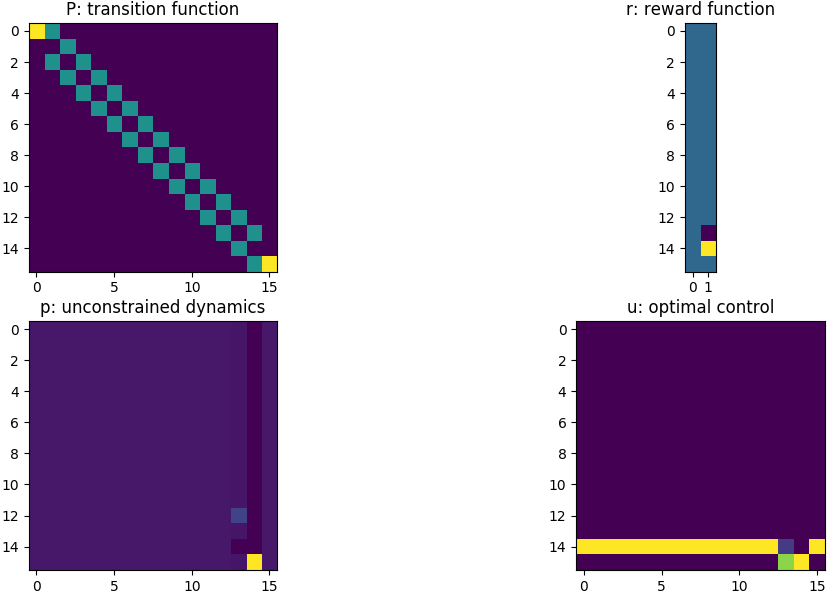
\includegraphics[width=0.65\textwidth,height=0.325\textheight]{../../pictures/figures/chain-test-zero-rewards.png}
\caption{A chain problem \cite{Sutton2018a} with zero reward on all states except the last two. A small negative reward, then a large positive one.
The optimal control to this problem is not realisable: in every state, jump to the state with positive reward.}
\label{fig:chain-zero}
\end{figure}

\begin{figure}
\centering
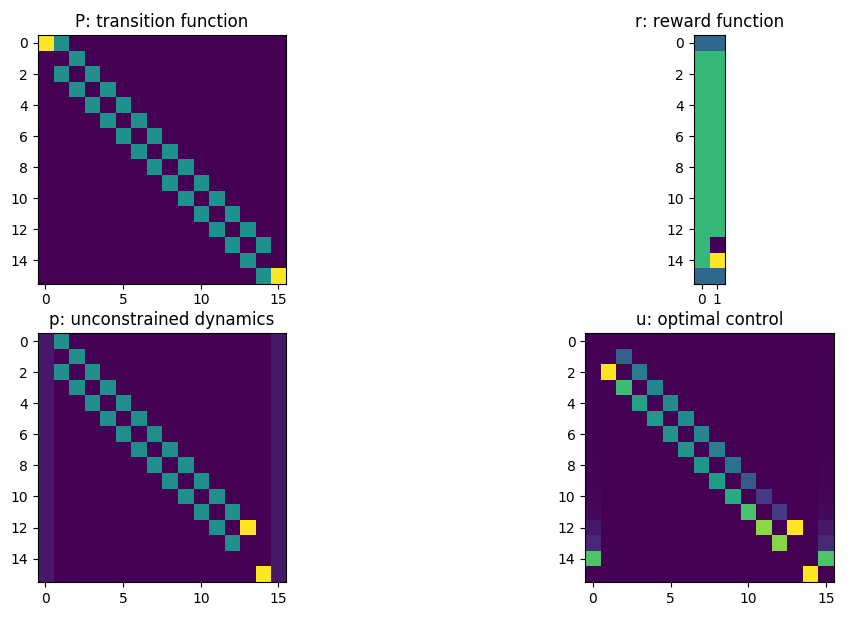
\includegraphics[width=0.65\textwidth,height=0.325\textheight]{../../pictures/figures/chain-test-pos-rewards.png}
\caption{The same chain problem as above, but with an positive reward added to all states.
We can see that the structure of the transition function has now made it into the optimal control!
The LMDP's control can be decoded into a realisable policy.}
\label{fig:chain-pos}
\end{figure}

\subsection{Discussion}\label{lmdp-validation}

Unfortunately, Todorov \cite{Todorov2006,Todorov2009} never actually produced
any experiments that use the linear bellman equation to solve a MDP.
His experiments were with $Z$-learning, the linearised counterpart to $Q$-learning.

\begin{align*}
\tilde z(s) = e^{q(s)}z(s{'})^{\gamma} \tag{linearised bellman eqn}\\
z_{t+1}(s_i) = (1- \eta)z_{t}(s_i) + \eta\tilde z(s_i) \tag{$Z$ iteration}\\
\end{align*}

He makes this work by hand picking $q$ so that the optimisation will converge to the optimal value.
Then he evaluates the accuracy of the value estimates.
They do not give a general way of constructing $q$ from a MDP that actually works (in the sense of yielding the same optima).
Nor do they give an efficient way to map an optimal control to an optimal policy.

% \begin{figure}
% \centering
% 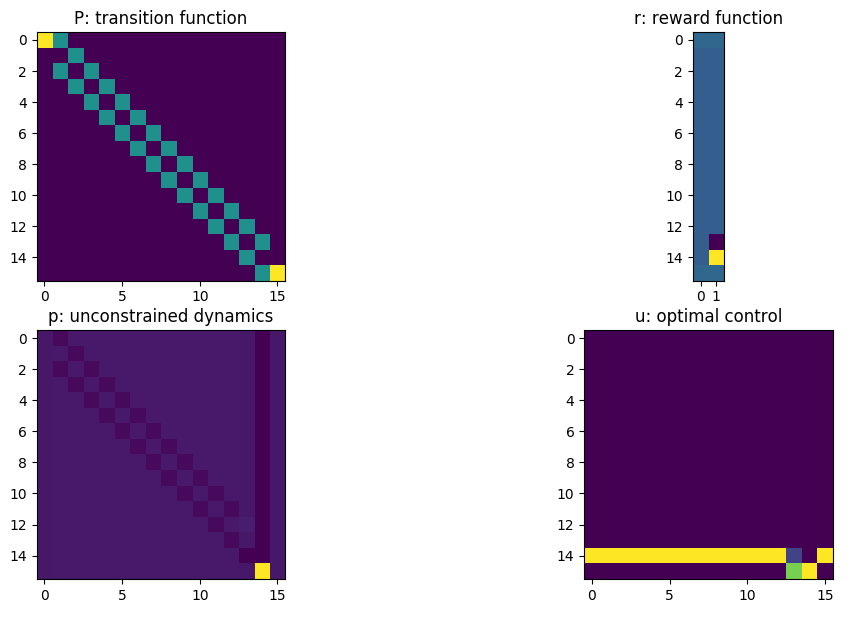
\includegraphics[width=1\textwidth,height=0.35\textheight]{../../pictures/figures/chain-test-neg-rewards.png}
% \caption{A chain problem with negative rewards applied to all states.
% Again, the structure of the transition function is missing.}
% \end{figure}

Because there are no benchmarks that we can validate our implementation on,
there is some doubt about whether I implemented the LMDP correctly. While the
LDMP solution strategy does occasionally pick the correct optimal policy, more often than not,
its guesses are seriously wrong.

\subsubsection{Linearity in MDPs}

Todorov's formulation of LMDPs does not seem to allow a MDP to be to reliably embed a LMDP.
Despite this, it might still be possible to construct a linear MDP given different assumptions.

Let's reconsider Jin et al.'s approach \cite{Wang}: construct a MDP where the value is a
linear function of a state-action representation and of a policy embedding.
It is important to note that, not every (policy) embedding can be realised as a policy, so to constrain the search dynamics properly
we must use the Bellman equation.

And this captures the essence of the problem. We need the Bellman equation for efficient search, but it is not linear in the policy.
So, we can linearise a MDP, but we will lose the ability to use the Bellman equation to guide the search for the optimal policy.

% Refs \cite{Todorov2006,Todorov2009,Zhong,Zhonga,Dvijotham,Wozabal}
% Linearise around the optimal policy. But how does that tell us how to act when not at the optimal policy?
